\begin{frame}
  \frametitle{Theory}

  \begin{columns}
    \begin{column}{0.5\textwidth}
      Theoretical basics:
      \begin{itemize}
        \item{MDP (Markov Decision Process),}
        \item{exploitation vs exploration,}
        \item{discounted rewards,}
        \item{Bellman equation,}
        \item{essential approaches:}
          \begin{itemize}
            \item{dynamic programming,}
            \item{Monte Carlo methods,}
            \item{temporal difference (TD) learning,}
          \end{itemize}
        \item{value functions,}
        \item{policy functions,}
      \end{itemize}
    \end{column}

    \begin{column}{0.35\textwidth}
      \begin{figure}
        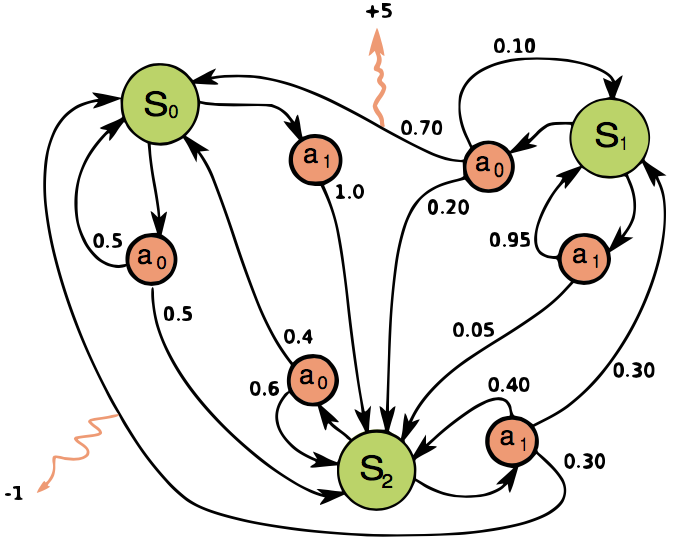
\includegraphics[width=\textwidth]{imgs/mdp.png}
        \caption{\tiny \textit{https://en.wikipedia.org/wiki/Markov\_decision\_process}}
      \end{figure}
    \end{column}
  \end{columns}

\end{frame}
